% !TEX TS-program = pdflatex
% !TEX encoding = UTF-8 Unicode

% This is a simple template for a LaTeX document using the "article" class.
% See "book", "report", "letter" for other types of document.

\documentclass[11pt]{article} % use larger type; default would be 10pt

\usepackage[utf8]{inputenc} % set input encoding (not needed with XeLaTeX)

%%% Examples of Article customizations
% These packages are optional, depending whether you want the features they provide.
% See the LaTeX Companion or other references for full information.

%%% PAGE DIMENSIONS
\usepackage{geometry} % to change the page dimensions
\geometry{a4paper} % or letterpaper (US) or a5paper or....
% \geometry{margin=2in} % for example, change the margins to 2 inches all round
% \geometry{landscape} % set up the page for landscape
%   read geometry.pdf for detailed page layout information

\usepackage{graphicx} % support the \includegraphics command and options

% \usepackage[parfill]{parskip} % Activate to begin paragraphs with an empty line rather than an indent

%%% PACKAGES
\usepackage{booktabs} % for much better looking tables
\usepackage{array} % for better arrays (eg matrices) in maths
\usepackage{paralist} % very flexible & customisable lists (eg. enumerate/itemize, etc.)
\usepackage{verbatim} % adds environment for commenting out blocks of text & for better verbatim
\usepackage{subfig} % make it possible to include more than one captioned figure/table in a single float
% These packages are all incorporated in the memoir class to one degree or another...
\usepackage{natbib}

%%% HEADERS & FOOTERS
\usepackage{fancyhdr} % This should be set AFTER setting up the page geometry
\pagestyle{fancy} % options: empty , plain , fancy
\renewcommand{\headrulewidth}{0pt} % customise the layout...
\lhead{}\chead{}\rhead{}
\lfoot{}\cfoot{\thepage}\rfoot{}

%%% SECTION TITLE APPEARANCE
\usepackage{sectsty}
\allsectionsfont{\sffamily\mdseries\upshape} % (See the fntguide.pdf for font help)
% (This matches ConTeXt defaults)

%%% ToC (table of contents) APPEARANCE
\usepackage[nottoc,notlof,notlot]{tocbibind} % Put the bibliography in the ToC
\usepackage[titles,subfigure]{tocloft} % Alter the style of the Table of Contents
\renewcommand{\cftsecfont}{\rmfamily\mdseries\upshape}
\renewcommand{\cftsecpagefont}{\rmfamily\mdseries\upshape} % No bold!

\usepackage{fullpage}

%%% END Article customizations

%%% The "real" document content comes below...

\title{Summary of Ocean0-2\_COM\_MOM6 Results (sigma\_zstar)}
\author{Gustavo Marques, Alon Stern, Matthew Harrison, Olga Sergienko, \\ Alistair Adcroft and Robert Hallberg}

\begin{document}
\maketitle

\section{Model Details}

\begin{itemize}
\item Model and version: Modular Ocean Model v. 6 (MOM6).
\item Repository: https://github.com/gustavo-marques/MOM6/releases/tag/ISOMIP.v1.0 
\item Model configuration and input files: 
\begin{itemize}
   \item https://github.com/gustavo-marques/ISOMIP/tree/master/setup/Ocean0/COM/MOM\_override.sigma\_zstar
   \item https://github.com/gustavo-marques/ISOMIP/tree/master/setup/Ocean1/COM
   \item https://github.com/gustavo-marques/ISOMIP/tree/master/setup/Ocean2/COM
   \item Note: for the sigma\_zstar experiments MOM\_override.sigma\_zstar must be used.
\end{itemize}
\item Vertical coordinate: following \cite{Stern2017}, we employ a coordinate system that is a hybrid between a z$^*$ and a terrain-following coordinate. Outside the ice shelf cavity, the vertical coordinate is defined by the $z^*$ formulation proposed by \cite{Adcroft2004}. However, within the cavity, model layers deform following the base of the ice shelf, as they would in a terrain-following coordinate, but with the fact that layers collapse to zero once they intersect the bottom topography, as in a $z^*$.
\item Horizontal mixing: harmonic (del2); along-isopycnal for diffusivities and along-layer for viscosity.
\item Vertical mixing: del2 with COM constant viscosity and diffusivity set as background values. Additional vertical mixing is also applied based on the parameterization developed by \cite{Jackson2008}, more details below. Within the mixed layer, vertical mixing is also controlled by the ocean boundary layer scheme described in \cite{Reichl2018}.
\item Advection schemes: momentum - second-order centered; tracers - piecewise linear method.
\item Equation of state: linear with ISOMIP+ coefficients.
\item Convection parameterization: based on the parameterization developed by \cite{Jackson2008} using a critical Richardson number of $Ri_c$ = 0.25.

\item Ocean boundary layer scheme: near-surface vertical mixing is parameterized with an energy consistent planetary boundary layer scheme \citep{Reichl2018}, with a minimum vertical viscosity of $10^{-2}$ m$^2$/s.

\item Melt parameterization: $T_w$, $S_w$ and $u_w$ were averaged within 20 m of the ice draft; $u_w$ was averaged the to the tracer grid using four horizontal neighbors. Melting was set to zero in regions where the ice depth was less than 90 m and when the total water column thickness was less than 10 m.

\item Modifications to Topography: Interpolated to 2-km grid using a spline method\footnote{http://docs.scipy.org/doc/scipy/reference/generated/scipy.interpolate.interp2d.html\#scipy.interpolate.interp2d} then smoothed the ice thickness using a Gaussian filter\footnote{http://docs.scipy.org/doc/scipy-0.16.1/reference/generated/scipy.ndimage.filters.gaussian\_filter.html} with half-width of 1 and 5 km for the y and x direction, respectively. An offline calving criterion was used where ice thinner than 100 m was removed. To minimize pressure gradient errors due to a step-like ice cliff, this criterion was not applied near the ice front, which remained smooth. A minimum thickness of $\sim$ 40 m was maintained by decreasing the ice thickness near the grounding line.  

\item Maintaining sea level: mass fluxes were used and no corrections were applied to maintain the sea level unchanged.  

\item Deviations from COM: the model deviated from the COM vertical mixing and convection parameterization. Instead of prescribing the COM vertical viscosity/diffusivity when the local stratification was unstable, we applied the parameterization developed by \cite{Jackson2008} using a critical Richardson number of $Ri_c$ = 0.25. Within the top boundary layer, vertical mixing is also controlled by the ocean boundary layer scheme described in \cite{Reichl2018}.

\item Parameter values:

\begin{tabular}{rl}
$\Gamma_T$ & $0.087$ \\
$\Gamma_S$ & $0.0087$ \\
$C_{D,\textrm{top}}$ & $2.5 \times 10^{-3}$
\end{tabular}
\end{itemize}

\begin{figure}[htbp]
\begin{center}
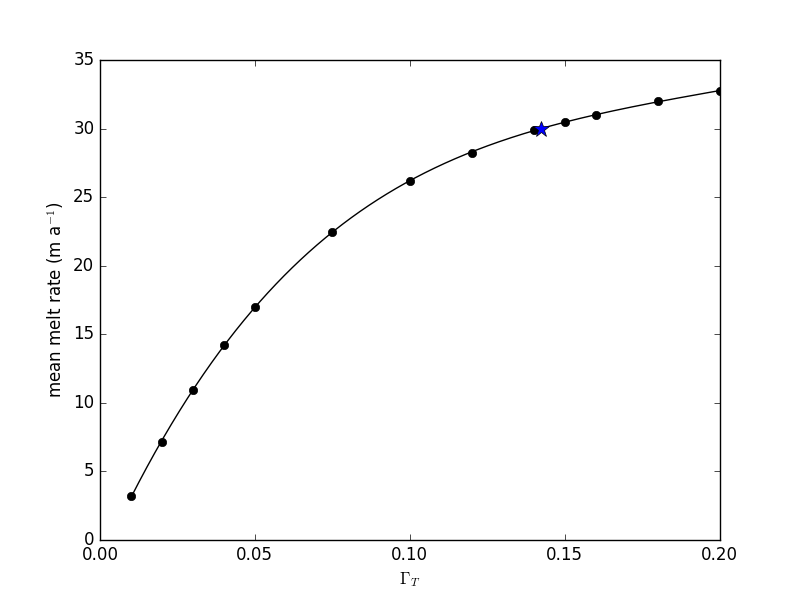
\includegraphics[scale=0.65]{python/melt_gamma_COM.png}
\label{fig1}
\caption{The dependence of the mean melt rate averaged over locations below $z_d$ = -300 m and over the final six months of the simulation for various values of the turbulent heat-transfer coefficient $\Gamma_T$ . Based on these results, the value of $\Gamma_T$ $\sim$ 0.087 (blue star), corresponding to a mean melt rate $m_w$ $\sim$ 30 m a$^{-1}$, was used in Ocean1 and Ocean2.}
\end{center}
\end{figure}


\bibliographystyle{te}


\bibliography{../../bib/refs}

\end{document}
